\documentclass[UTF8]{article}

% \usepackage{indentfirst} %缩进
% \usepackage{xeCJK}    %使用系统字体
\usepackage{ctex}
\usepackage{fancyhdr} %自定义页眉页脚
\usepackage{listings} %source code
\usepackage{tabu}
\usepackage{booktabs}
\usepackage{graphicx}
\usepackage{multirow}

% \setCJKmainfont{SimSun} %设置 CJK 主字体为 SimSun (宋体)
% \pagestyle{empty}                   %不设置页眉页脚
% \usepackage{amsmath, amsthm, amssymb, amsfonts} %数学公式
% \usepackage[a4paper,left=3cm,right=3cm,top=3cm,bottom=3cm]{geometry}
% %\usepackage[tmargin=1in,bmargin=1in,lmargin=1.25in,rmargin=1.25in]{geometry}.
% \usepackage{booktabs} %插入表格
% \usepackage[section]{placeins} %避免浮动
% \usepackage{listings} %插入代码
% \usepackage{ctex}     %中文宏包
% \usepackage[svgnames, table]{xcolor} %彩色表格
% \usepackage{algorithm}          %伪代码
% \usepackage{algorithmicx}
% \usepackage{algpseudocode}
% \usepackage{algorithm,algpseudocode,float}
% \usepackage{lipsum}
% \usepackage{enumitem}           %调整列举环境
% \usepackage{url}
% \usepackage{fontspec,xunicode}

% %-----------------------xeCJK下设置中文字体------------------------------%
% \setCJKfamilyfont{song}{SimSun}                             %宋体 song
% \newcommand{\song}{\CJKfamily{song}}
% \setCJKfamilyfont{fs}{FangSong}                      %仿宋  fs
% \newcommand{\fs}{\CJKfamily{fs}}
% \setCJKfamilyfont{ktgb}{KaiTi}                      %楷体2312 ktgb
% \newcommand{\ktgb}{\CJKfamily{ktgb}}
% \setCJKfamilyfont{yh}{Microsoft YaHei}                    %微软雅黑 yh
% \newcommand{\yh}{\CJKfamily{yh}}
% \setCJKfamilyfont{hei}{SimHei}                              %黑体  hei
% \newcommand{\hei}{\CJKfamily{hei}}
% \setCJKfamilyfont{hwxk}{STXingkai}                                %华文行楷  hwxk
% \newcommand{\hwxk}{\CJKfamily{hwxk}}

% \newcommand{\shiyanbaogao}{\fontsize{36pt}{\baselineskip}\selectfont}
% \newcommand{\chuhao}{\fontsize{42pt}{\baselineskip}\selectfont}     %初号
% \newcommand{\xiaochuhao}{\fontsize{36pt}{\baselineskip}\selectfont} %小初号
% \newcommand{\yihao}{\fontsize{28pt}{\baselineskip}\selectfont}      %一号
% \newcommand{\erhao}{\fontsize{21pt}{\baselineskip}\selectfont}      %二号
% \newcommand{\xiaoerhao}{\fontsize{18pt}{\baselineskip}\selectfont}  %小二号
% \newcommand{\sanhao}{\fontsize{15.75pt}{\baselineskip}\selectfont}  %三号
% \newcommand{\sihao}{\fontsize{14pt}{\baselineskip}\selectfont}       %四号
% \newcommand{\xiaosihao}{\fontsize{12pt}{\baselineskip}\selectfont}  %小四号
% \newcommand{\wuhao}{\fontsize{10.5pt}{\baselineskip}\selectfont}    %五号
% % \newcommand{\xiaowuhao}{\fontsize{9pt}{\baselineskip}\selectfont}   %小五号
% % \newcommand{\liuhao}{\fontsize{7.875pt}{\baselineskip}\selectfont}  %六号
% % \newcommand{\qihao}{\fontsize{5.25pt}{\baselineskip}\selectfont}    %七号
\begin{document}


\begin{titlepage}
\center{北京理工大学\underline{计算机}学院2017级}
\vspace{1cm}
\center{\Huge{《数字逻辑》实验一}}
\vspace{0.5cm}
\center{\Huge{实~验~报~告}}
\vspace{2cm}

\begin{center}
\begin{large}
\begin{tabular}{r c}
小组编号& xxxxx\\
\cline{2-2}\\
\hline
学\qquad 号& \hspace{1.7cm}{xxxx} \\
\cline{2-2}\\
姓\qquad 名& 你的名字 \\
\cline{2-2}\\
\hline
学\qquad 号& \hspace{1.7cm}{xxxx} \\
\cline{2-2}\\
姓\qquad 名& 你的名字 \\
\cline{2-2}\\ 
\hline
学\qquad 号& \hspace{1.7cm}{xxxx} \\
\cline{2-2}\\
姓\qquad 名& 你的名字 \\
\cline{2-2}\\ 



\end{tabular}
\end{large}
\end{center}
\vfill \hfill
\end{titlepage}
\clearpage


\section{设计题目}

\begin{center}
    
\center{可调速循环流水灯}
\end{center}

\section{设计目的}

1、熟悉一次完整的FPGA开发流程,从新建工程,代码设计,综合实现,管脚约束,下载FPGA程序。
2、熟悉Xilinx Vivado开发环境,Verilog语言编程基本框架。
3、熟悉EES-338口袋计算机硬件平台。

每次上电,按一下rst复位键,LED0~LED7全亮,按住run键,则流水灯从左向右滚动,滚到最右,自动向左滚,滚到左侧,再向右滚动,周而复始。
在循环流水灯基础上,可以通过设计按键调整LED灯的亮灯时间,实现变速流水灯。


\section{设备器材}
Xilinx Vivado开发环境

EES-338口袋计算机硬件平台,配备 FPGA (XC7A35TCSG324-1C)

\section{设计原理与内容}

状态机图
模块化思想
边沿检测


\section{设计步骤}
\subsection{描述需求}

led灯一共有9个状态,需要控制状态转换的信号(move)以及使信号有效的使能(run)。速度等级level由btnup btndown分别控制。
\subsection{定义输入与输出}

\begin{figure}[htbp]
    \centering
    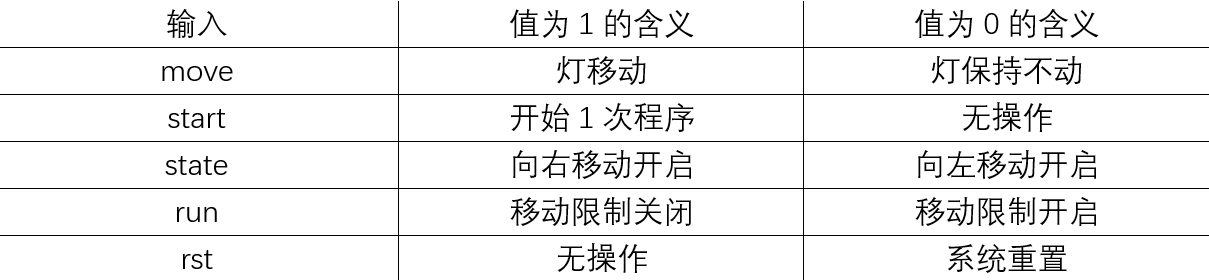
\includegraphics[scale=0.7]{流水灯控制输入变量.PNG}
    \caption{流水灯控制输入变量}
\end{figure}

\begin{figure}[htbp]
    \centering
    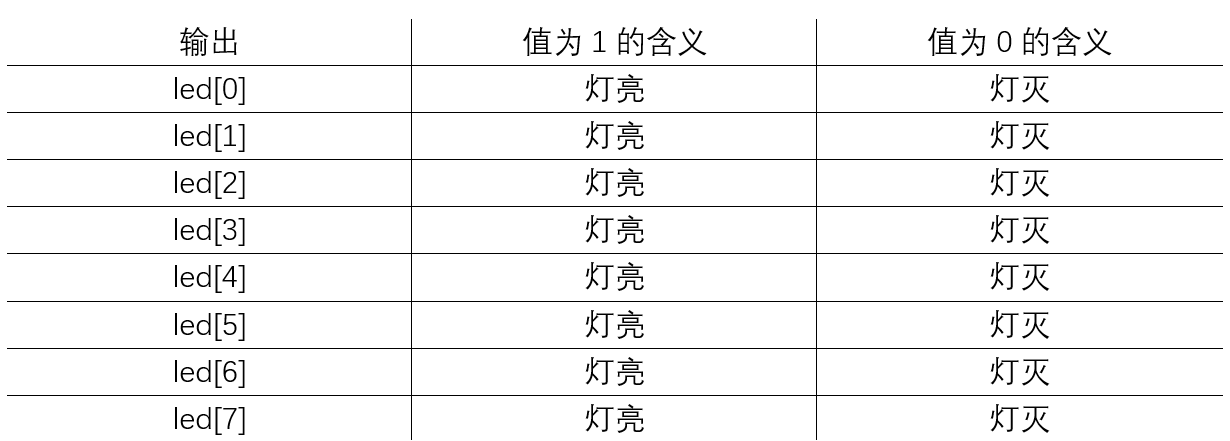
\includegraphics[scale=0.7]{流水灯输出变量.PNG}
    \caption{流水灯输出变量}
\end{figure}


% GRAGH
\subsection{状态机图}
% GRAGH

\begin{figure}[htbp]
    \centering
    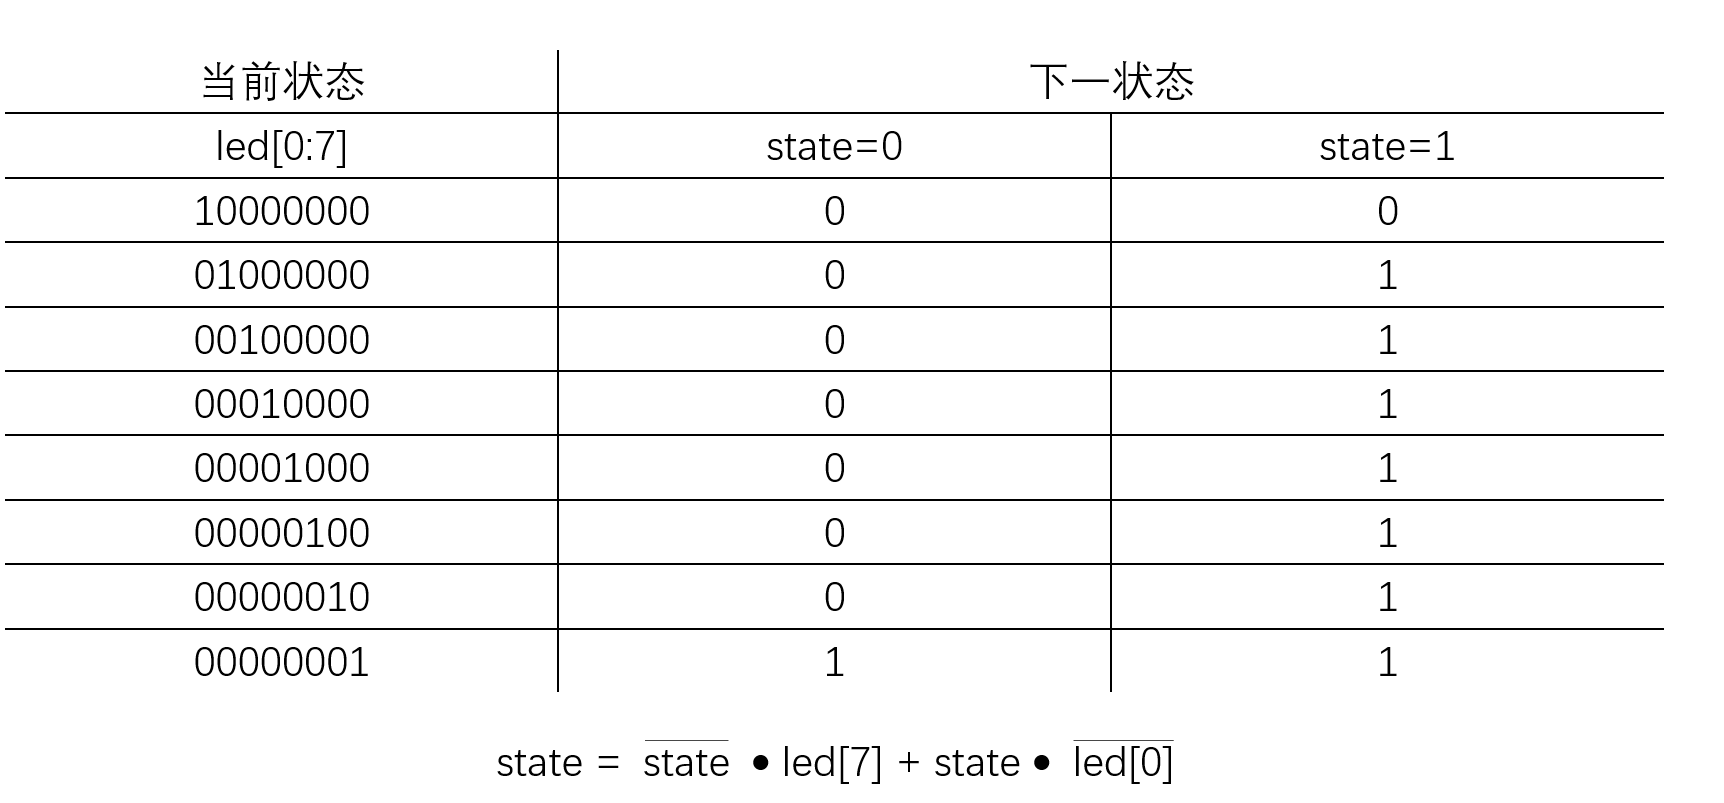
\includegraphics[scale=0.6]{state状态表及布尔表达式.PNG}
    \caption{state状态表及布尔表达式}
\end{figure}

\begin{center}  
\begin{figure}[htbp]
    % \centering
    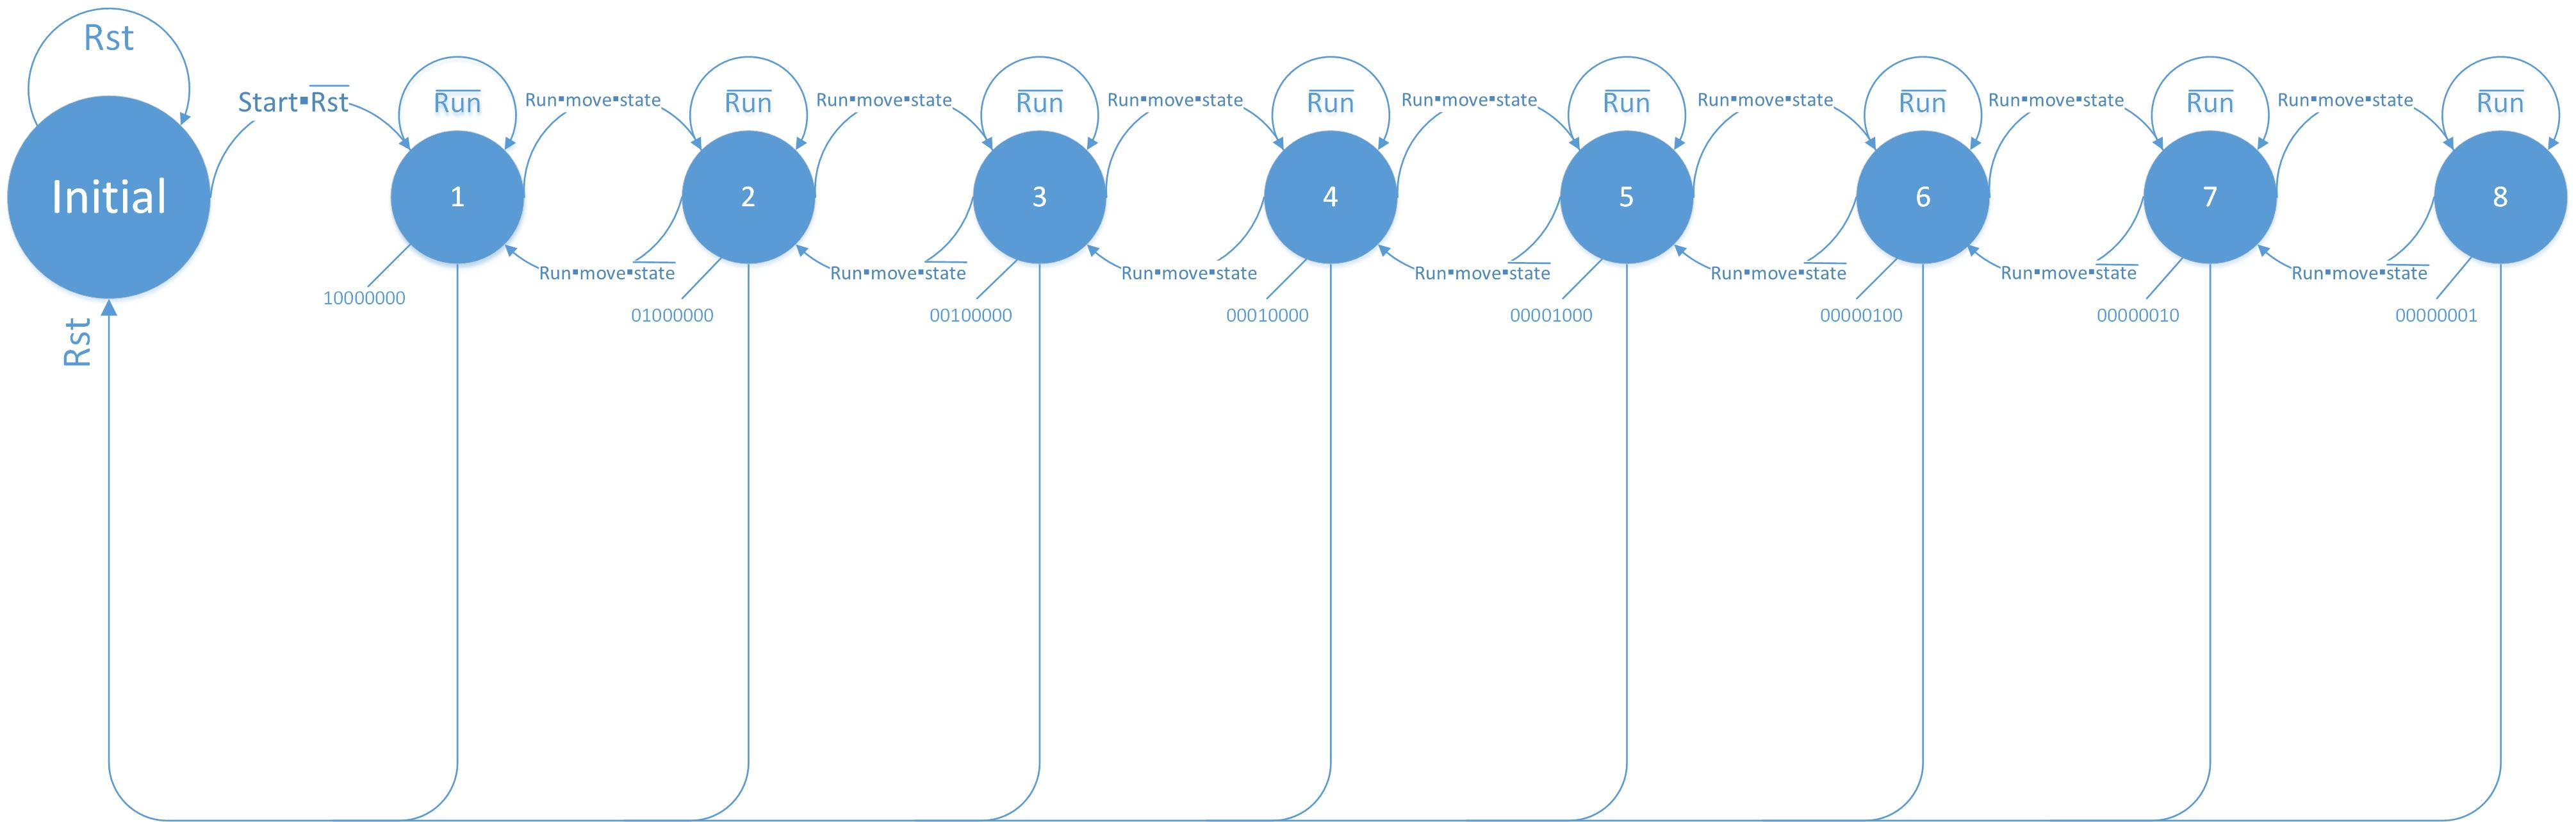
\includegraphics[scale=0.25]{状态机图.jpg}
    \caption{状态机图}
\end{figure}
\end{center}
\subsection{程序实现}

% code

\subsection{仿真与测试}
\subsubsection{各模块RTL图}
\begin{figure}[htbp]
    \centering
    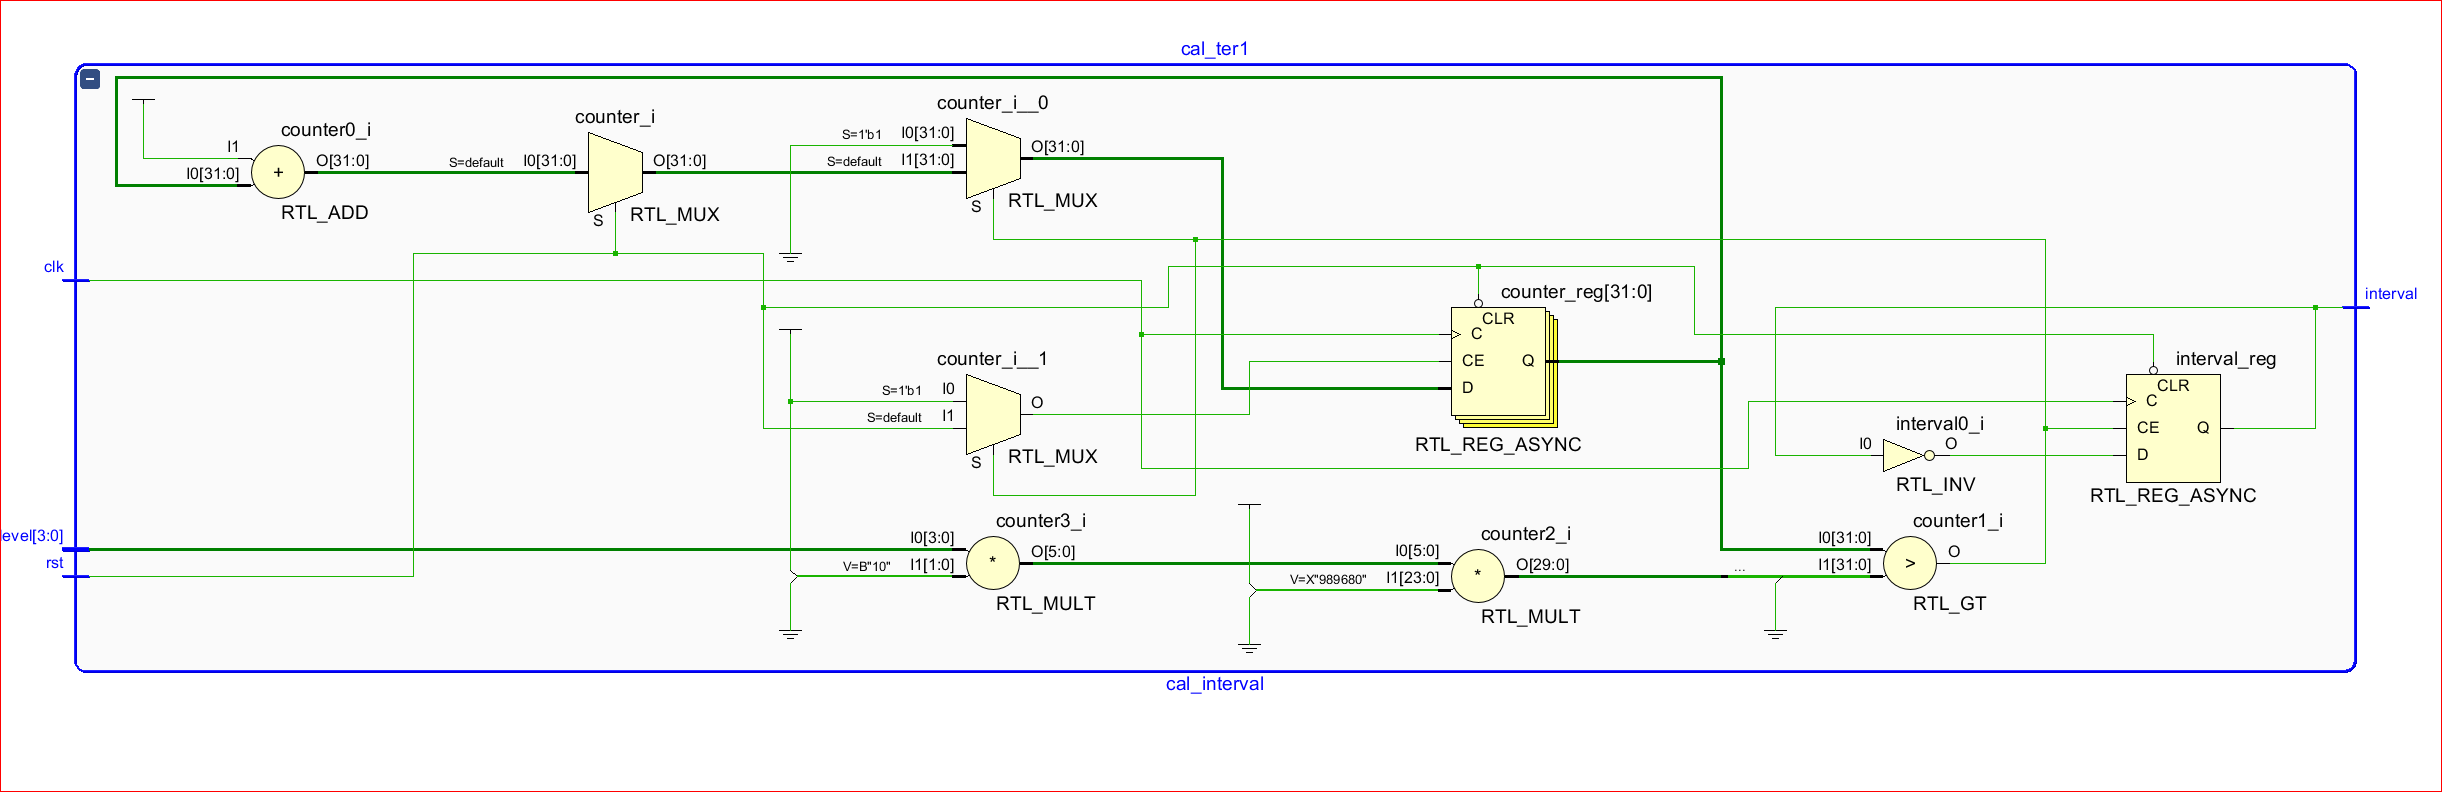
\includegraphics[scale=0.45]{cal_interval.PNG}
    \caption{cal interval}
\end{figure}

\begin{figure}[htbp]
    \centering
    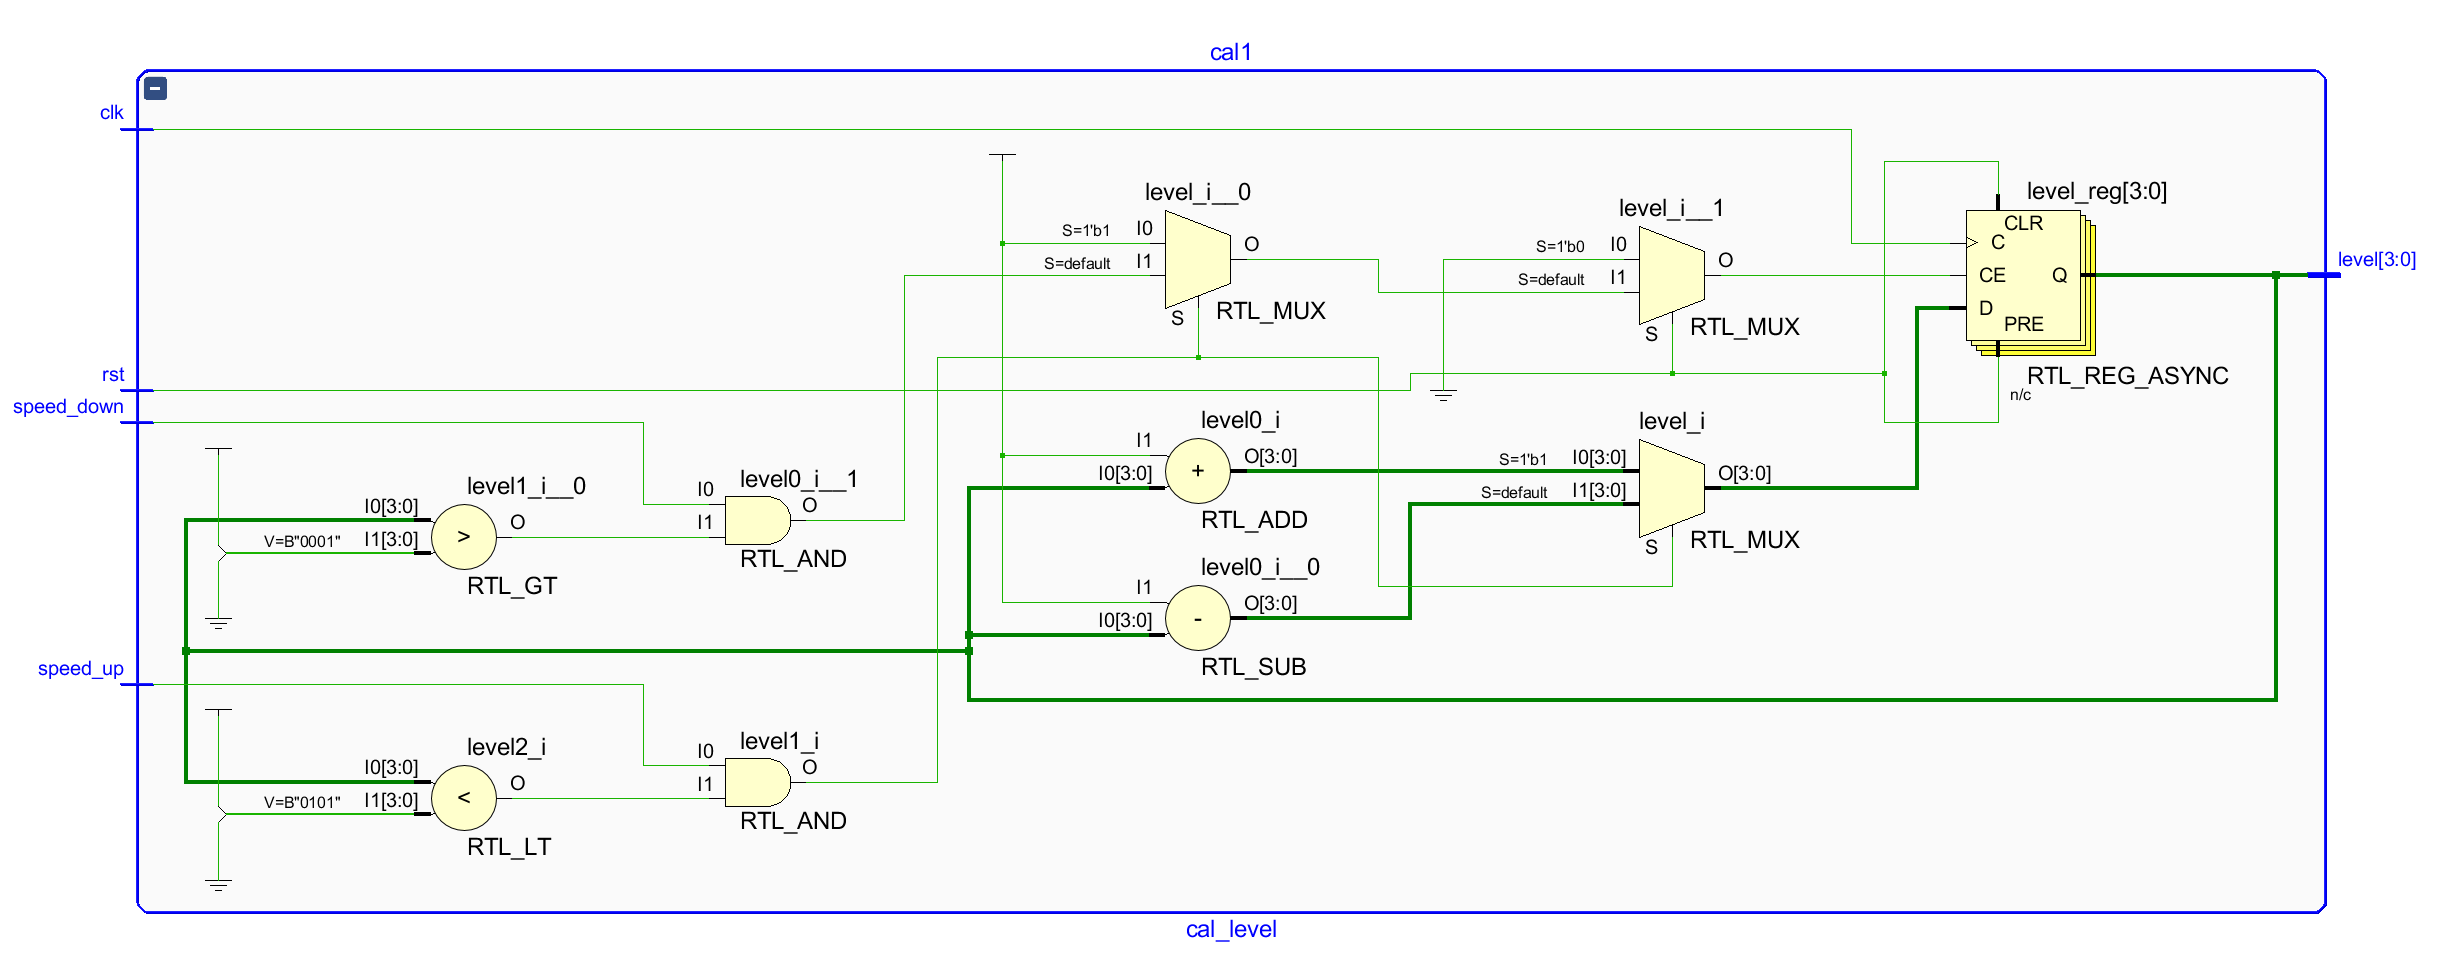
\includegraphics[scale=0.45]{cal_level.PNG}
    \caption{cal level}
\end{figure}

\begin{figure}[htbp]
    \centering
    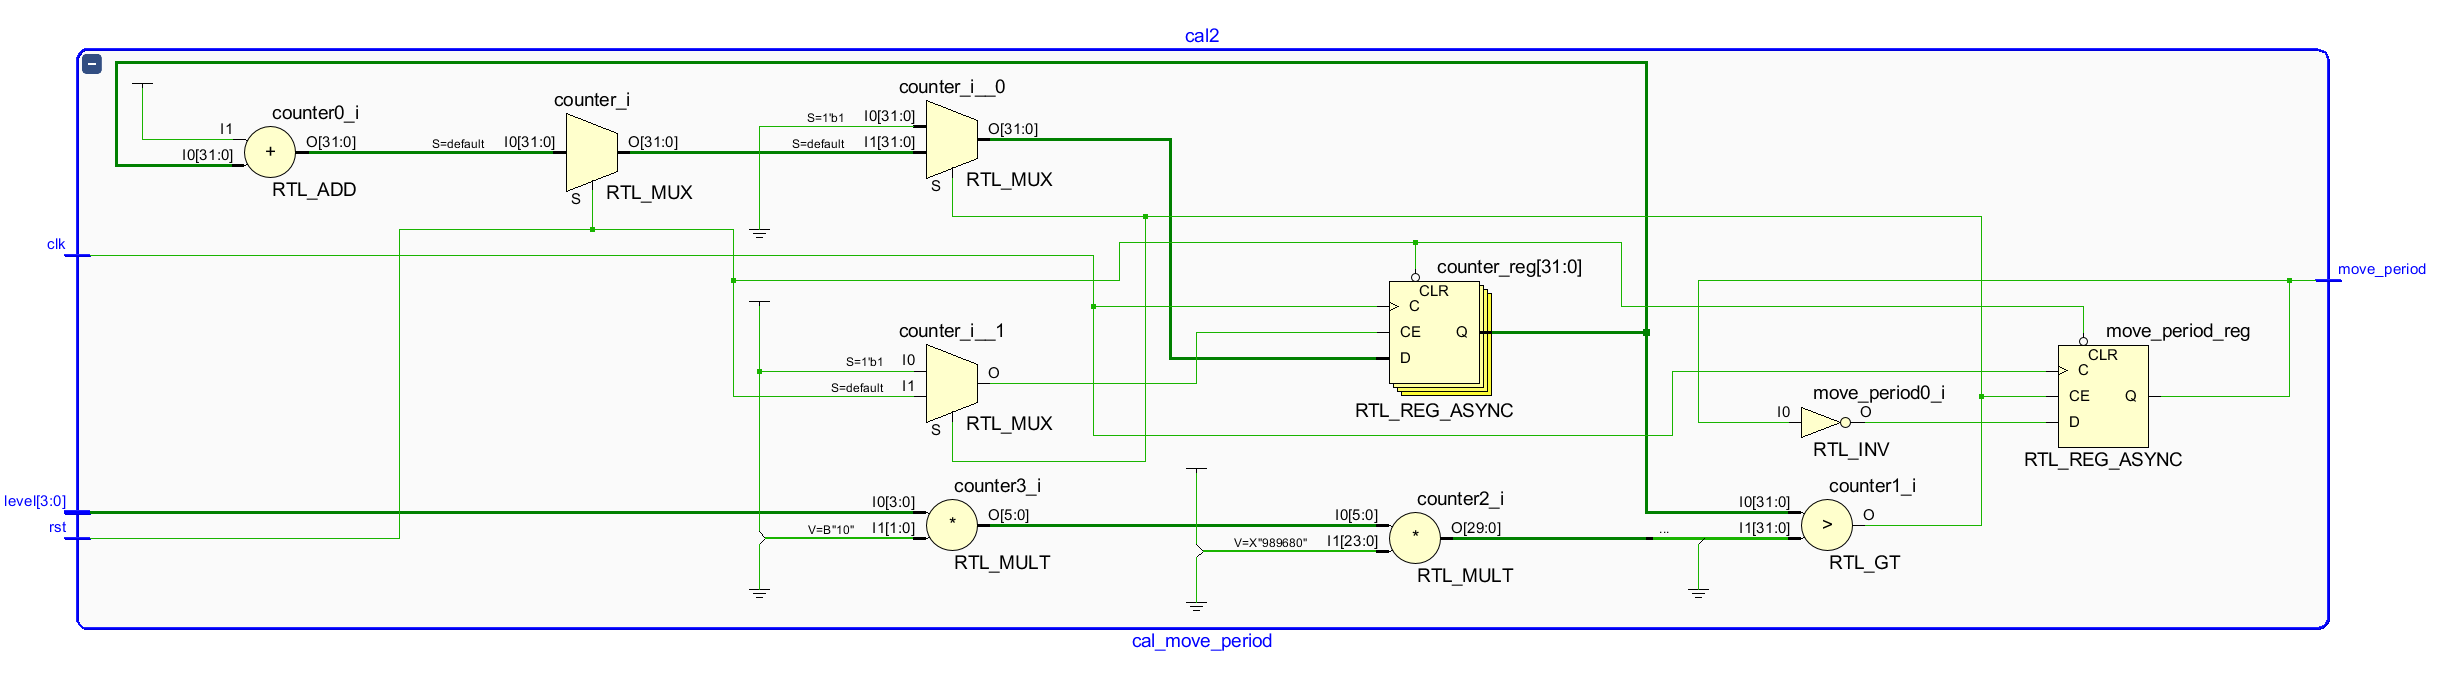
\includegraphics[scale=0.45]{cal_move_period.PNG}
    \caption{cal move period}
\end{figure}

\begin{figure}[htbp]
    \centering
    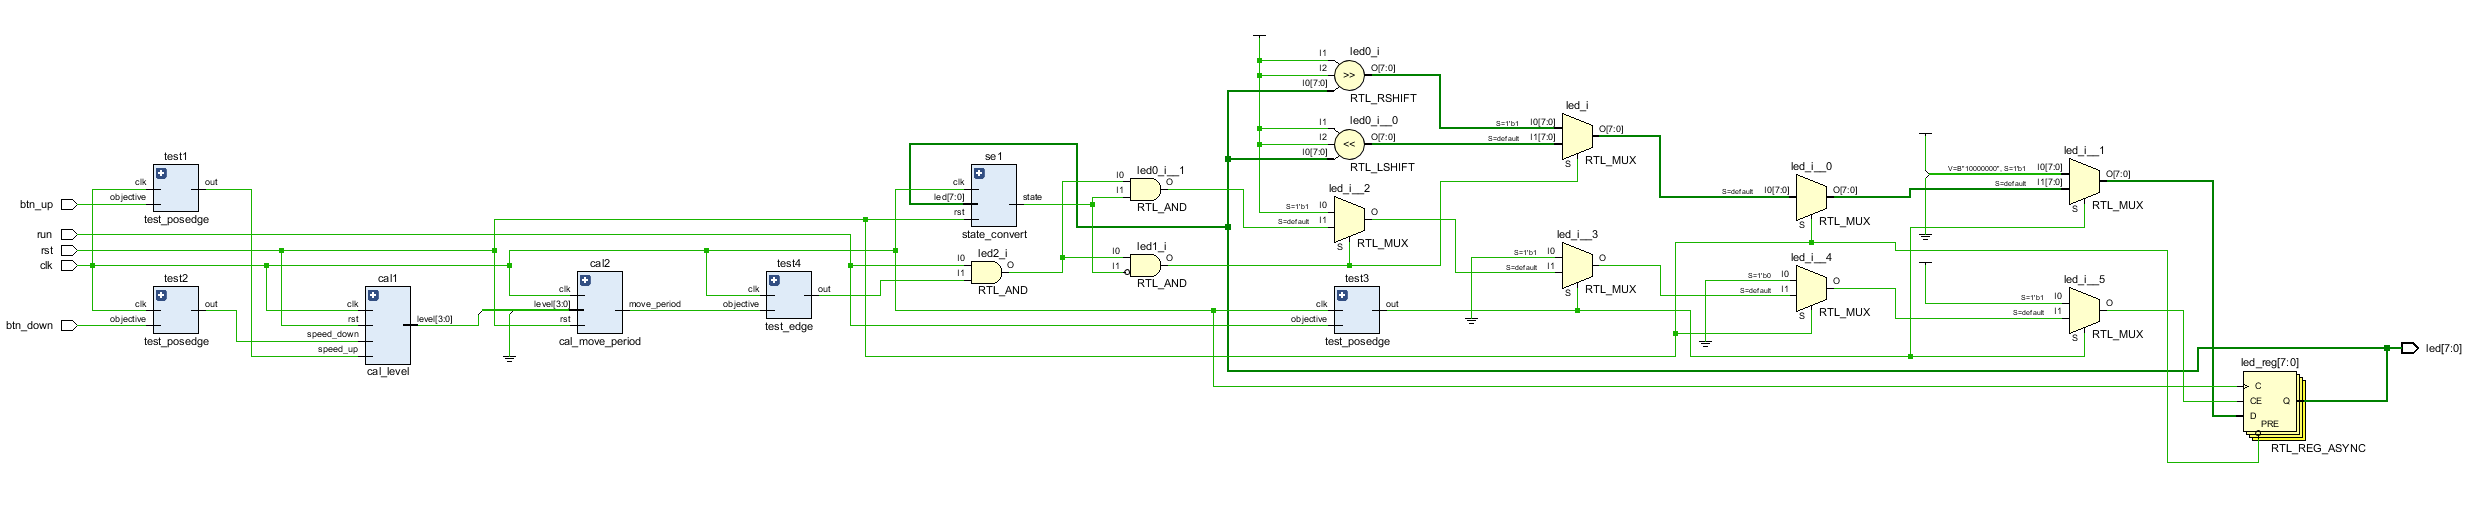
\includegraphics[scale=0.45]{overall.PNG}
    \caption{overall}
\end{figure}

\begin{figure}[htbp]
    \centering
    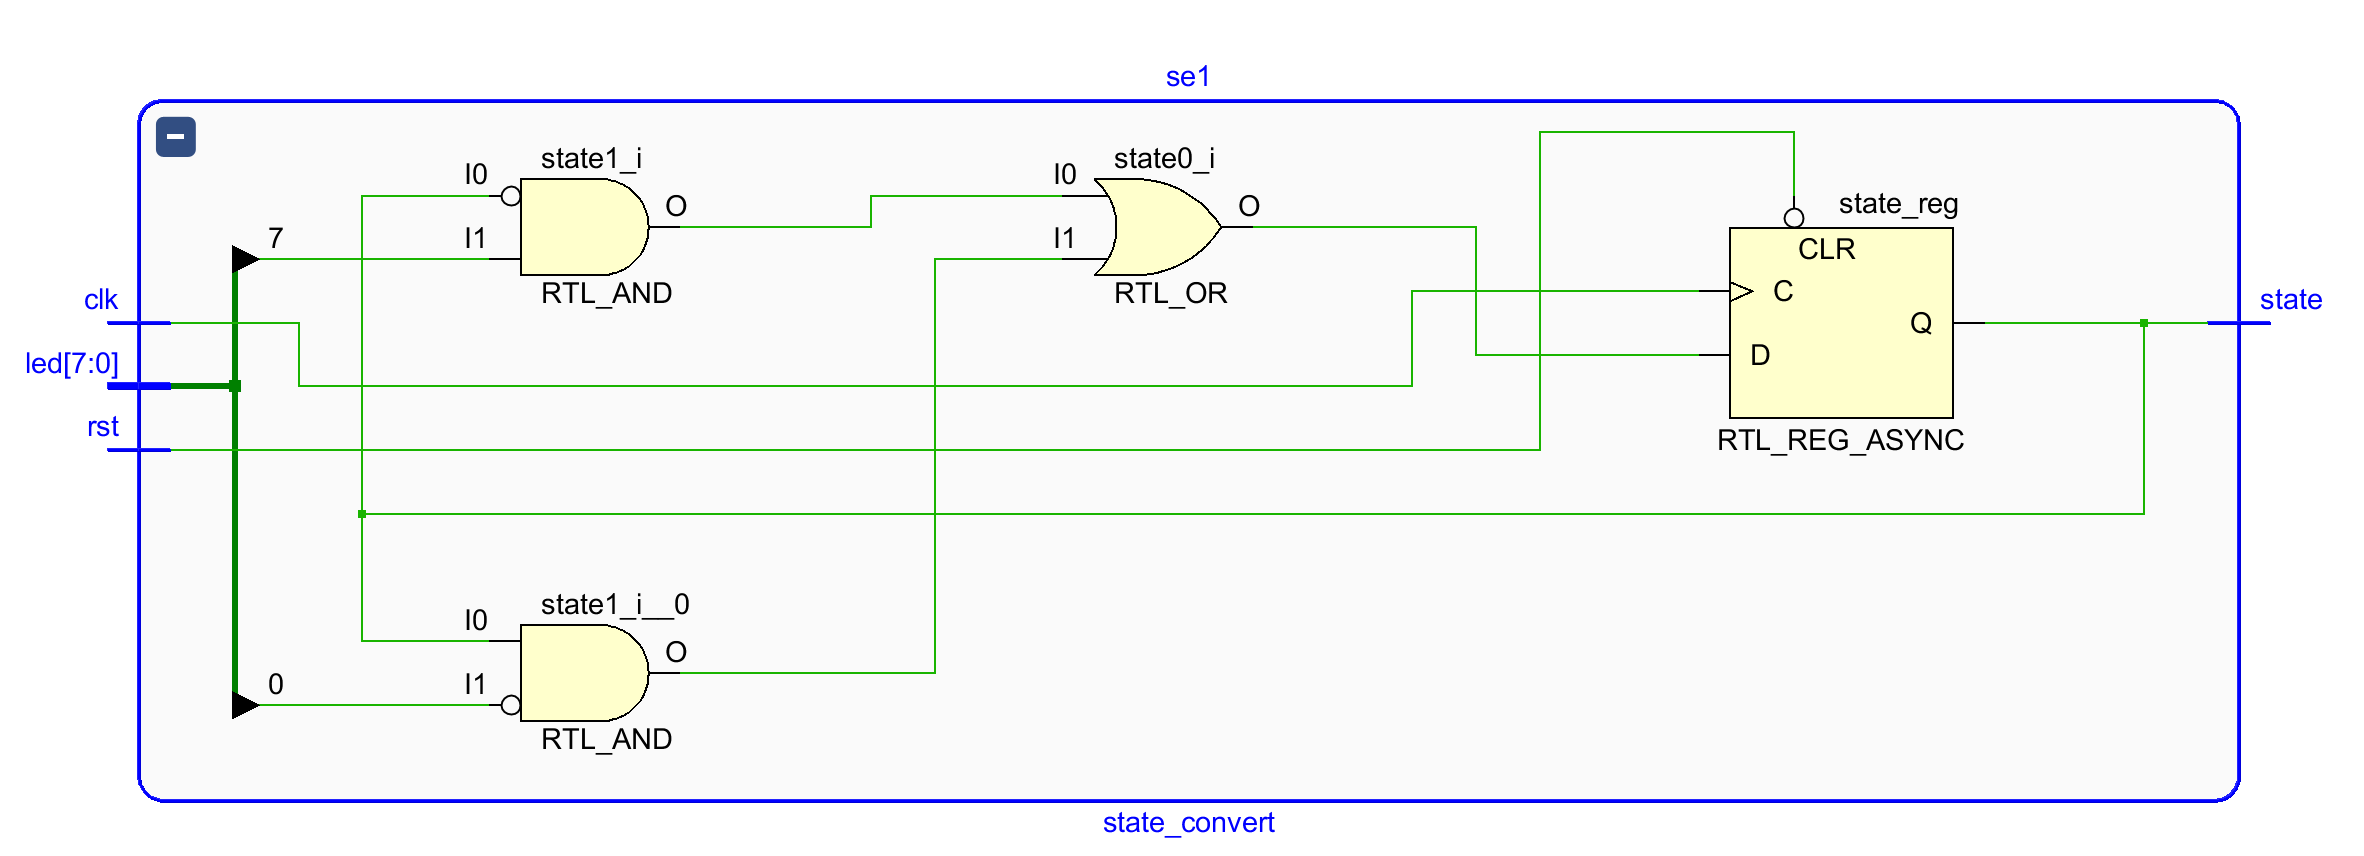
\includegraphics[scale=0.45]{state_convert.PNG}
    \caption{state convert}
\end{figure}
\subsubsection{测试}
\begin{figure}[htbp]
    \centering
    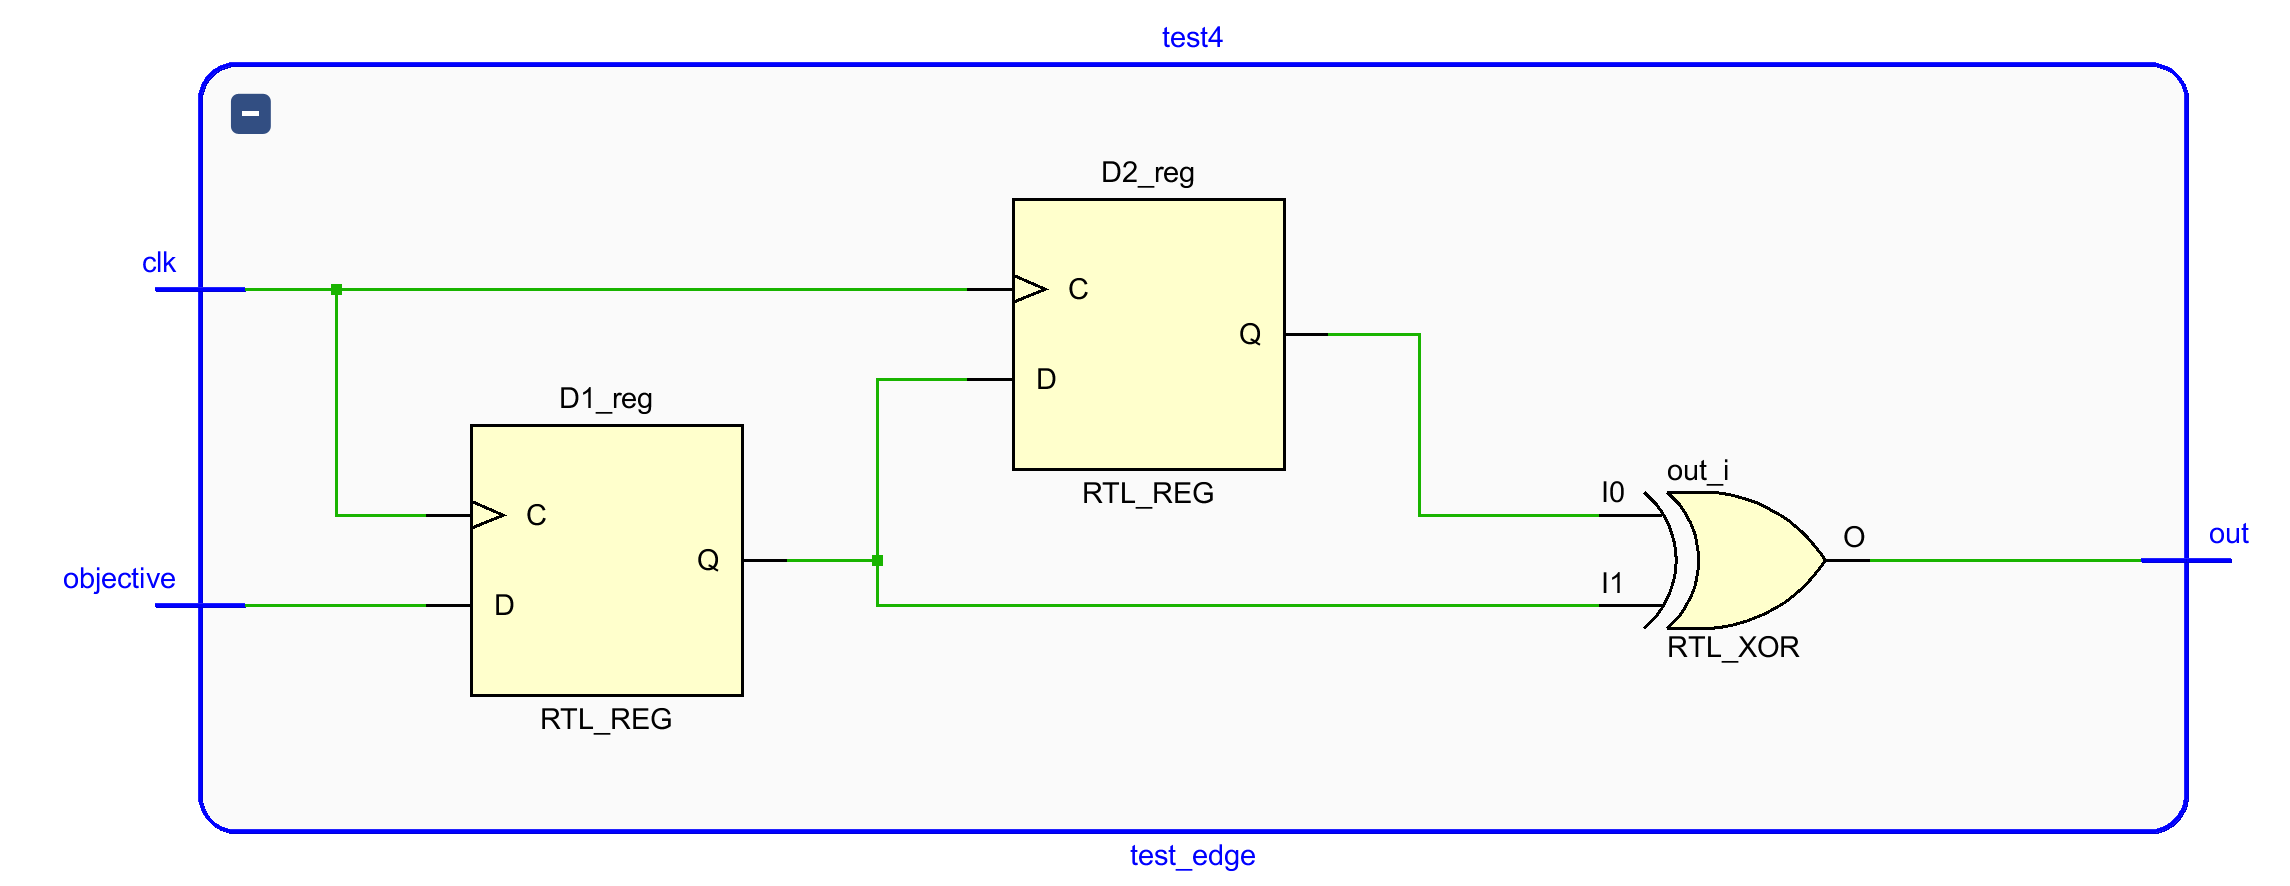
\includegraphics[scale=0.45]{test_edge.PNG}
    \caption{test edge}
\end{figure}
\begin{figure}[htbp]
    \centering
    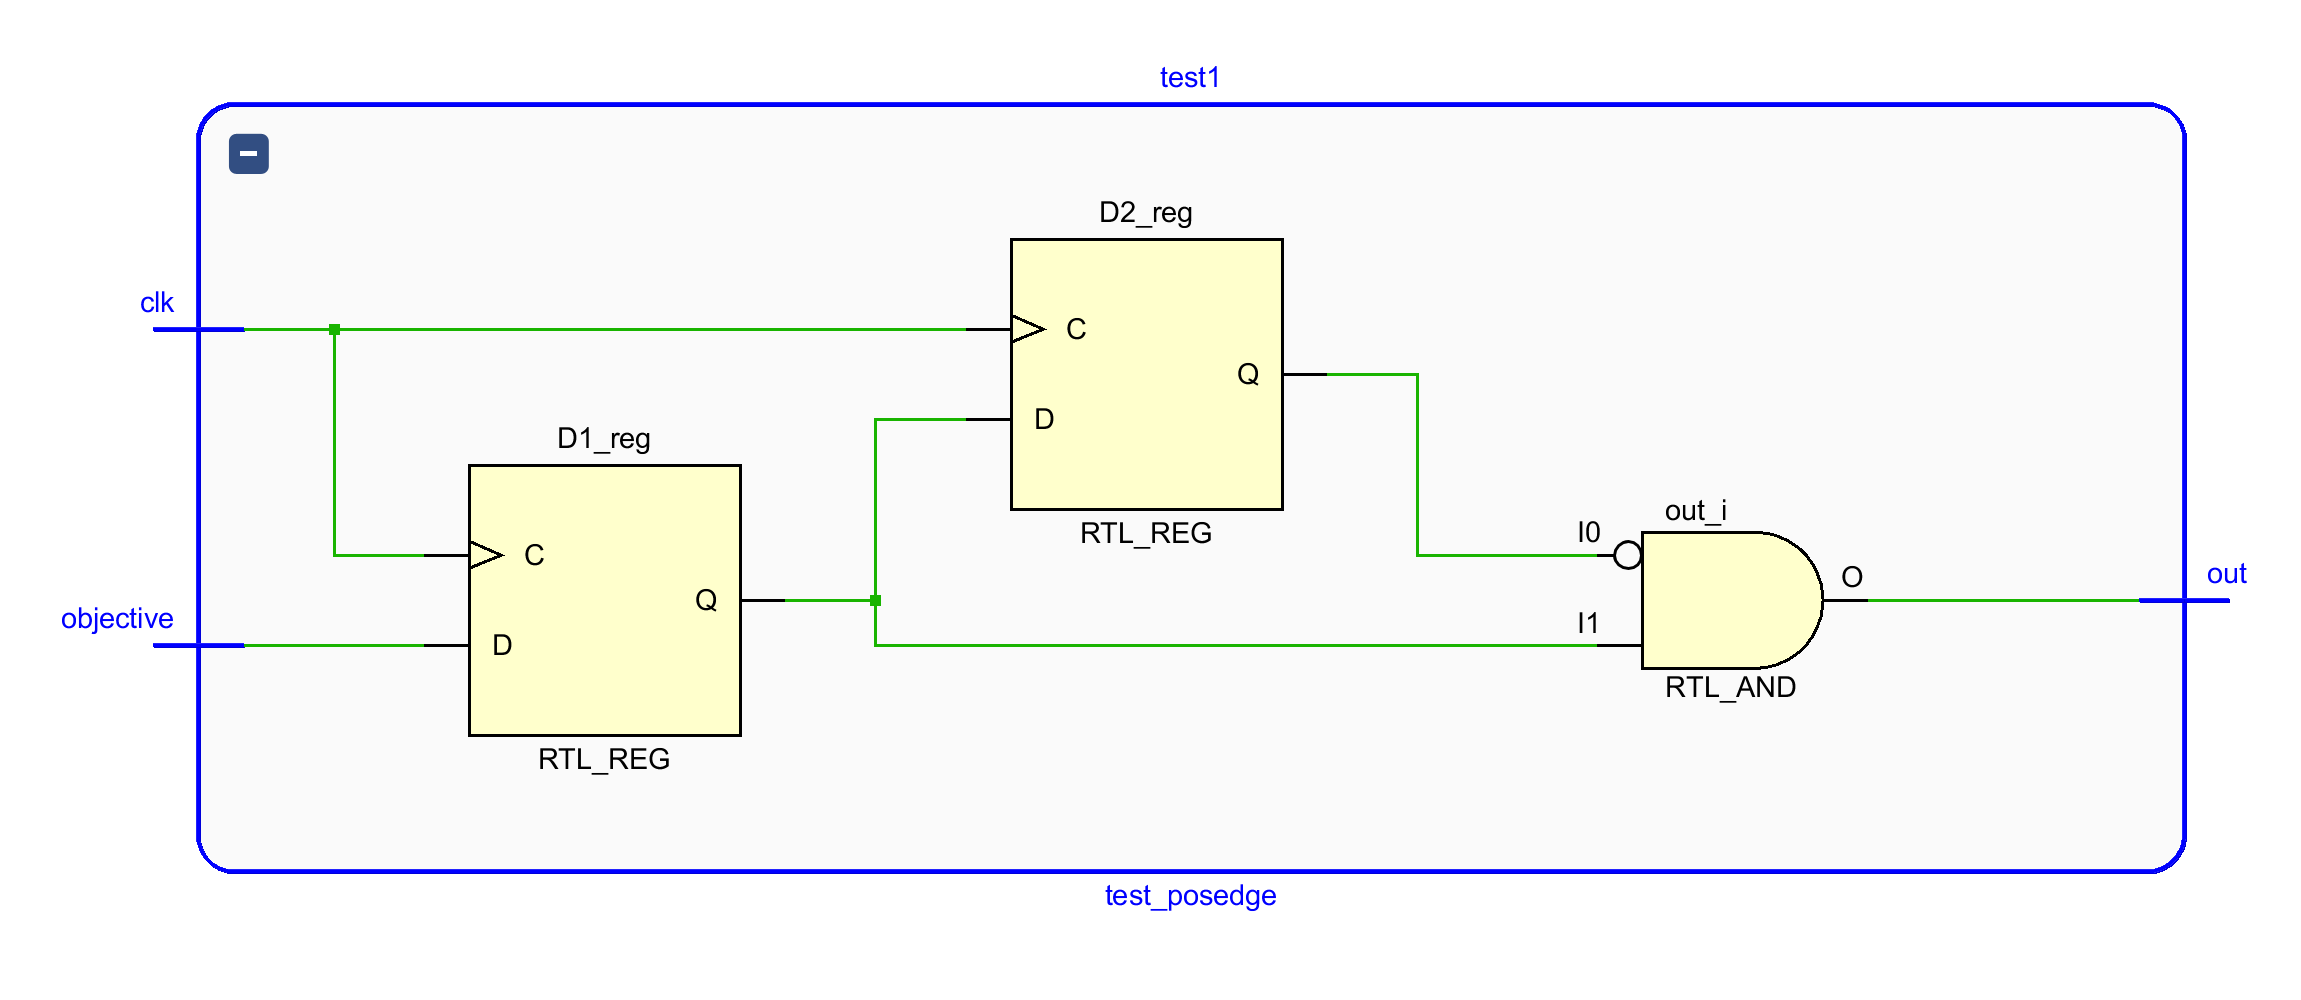
\includegraphics[scale=0.45]{test_posedge.PNG}
    \caption{test posedge}
\end{figure}
\subsection{综合与实现}
\subsection{生成mcs文件烧录到flash}
\subsection{运行结果显示}
\section{遇到的问题及解决方法}
\subsection{Ambiguous clock in event control}

https://stackoverflow.com/questions/27145548/ambiguous-clock-in-event-control

问题原因: 

一个时序电路always语句块里可能有两个条件同时满足比如
    if A则B
    if C则D
AC可能同时为真则可能进入两个逻辑之中

\subsection{stimulation error}
问题原因:

模块

\end{document}
